This examples is implemented for validating that the ROMC
implementation works accurately in a multidimensional parameter
space.

\subsubsection*{Problem Definition}

The equations describing this inference problem are presented below.

\begin{gather} \label{eq:ex1_equations}
  p(\thetab) = p(\theta_1)p(\theta_2)
  = \mathcal{U}(\theta_1; -2.5, 2.5) \mathcal{U}(\theta_2; -2.5, 2.5)\\
  p(\yb|\thetab) = \mathcal{N}(\yb;\thetab, \mathcal{I})\\
  p(\thetab|\yb) = \frac{1}{Z}p(\thetab)p(\yb|\thetab)\\
  Z = \int_{\thetab} p(\thetab)p(\yb|\thetab) d\thetab
\end{gather}

\noindent
In this simple example, it is feasible to evaluate the likelihood and
the unnormalised posterior. Additionally, the partition function $Z$
can be estimated by numerical integration (i.e. using Riemann's
approximation). Hence, it is feasible to compute the ground-truth
posterior with numerical approximation. Setting the observation
$\data$ to $(-0.5,0.5)$, the ground-truth posterior is illustrated in
figure \ref{fig:ex2_4}. In table \ref{tab:ex2}, we present the
ground-truth statistics i.e.\ $\mu, \sigma$ of the marginal posterior
distributions.

\subsubsection*{Performing the inference}

We perform the inference using the following hyperparameters
$n_1=500, n_2=30, \epsilon=0.4$. This set-up leads to a total of
$15000$ samples. As observed in the histogram of distances (figure
\ref{fig:ex2_1}), in the gradient-based approach, all optimisation
problems reach an almost zero-distance end point; hence all optimal
points are accepted. In the Bayesian optimisation scheme, the vast
majority of the optimisation procedures has the same behaviour; there
are only 4 optimal distances above the limit. In figure
\ref{fig:ex2_2}, the acceptance area of a specific optimisation
problem is demonstrated. We observe that both optimisation schemes
lead to a similar bounding box construction. This specific example is
representative of the rest of the optimisation problems; due to the
simplicity of the objective function, in most cases the optimal points
are similar and the surrogate model represents accurately the local
region. Hence, similar proposal regions are obtained by the two
optimisation alternatives.

The histograms of the marginal distributions, based on the weighted
samples, are presented in figure \ref{fig:ex2_3}. In the same figure,
we also plot the ground-truth distribution with the red dotted
line. We observe that the weighted samples follow quite accurately the
ground-truth distribution. This is also confirmed by the statistics
provided in table \ref{tab:ex2}; the sample mean $\mu$ and standard
deviation $\sigma$ are similar to the ground-truth for both parameters
$\theta_1$ and $\theta_2$. We also observe that both optimisation
schemes produce accurate samples.

Finally, the ground-truth and the approximate posteriors are presented
in figure \ref{fig:ex2_4}. We also confirm that the approximations are
close to the ground truth posteriors. As a note, we can observe that
the approximate posteriors present a diamond-shape in the mode of the
posterior; this happens due to the approximation of the circular
Gaussian-shape posterior with a sum of square boxes. The divergence
between the ground-truth distribution and the approximate ones is
$0.077$, using the Jensen-Shannon distance, which confirms the
satisfying matching between the two posteriors.

In this experiment we observed that the implementation fulfilled the
theoretical expectations for the ROMC inference method.

\begin{center} \label{tab:ex2}
\begin{tabular}{ c|c|c|c|c|c }
\hline
& $\mu_{\theta_1}$ & $\sigma_{\theta_1}$ & $\mu_{\theta_2}$ & $\sigma_{\theta_2}$ & Divergence\\
\hline \hline
Ground-truth & -0.45 & 0.935 & 0.45 & 0.935 & \\
\hline
ROMC (gradient-based) & -0.474 & 0.994 & 0.502 & 0.966 & 0.068\\
\hline
ROMC (Bayesian optimisation) & -0.485 & 0.987 & 0.511 & 0.939 & 0.069\\
\hline
\end{tabular}
\end{center}


\begin{figure}[ht]
    \begin{center}
      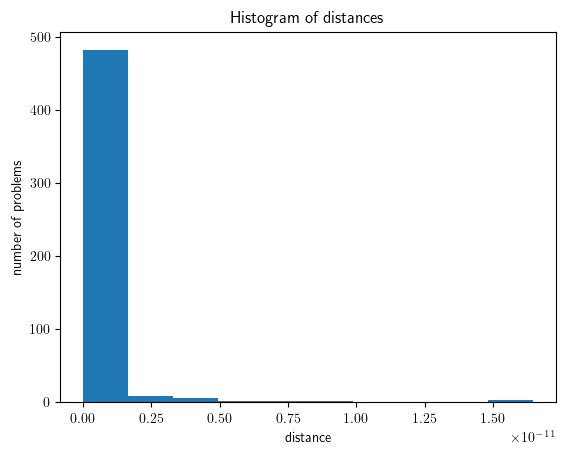
\includegraphics[width=0.48\textwidth]{./Thesis/images/chapter4/ex2D_distance_hist.png}
      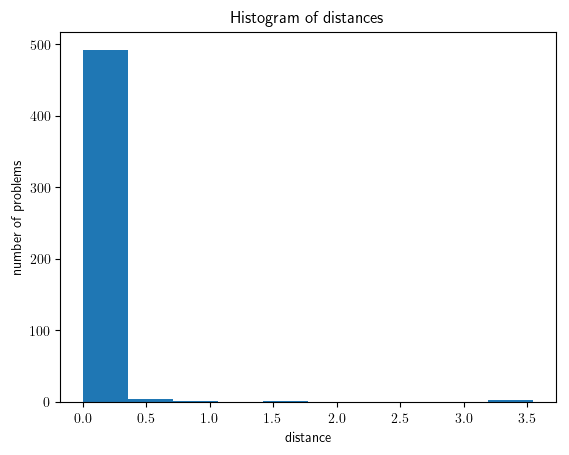
\includegraphics[width=0.48\textwidth]{./Thesis/images/chapter4/ex2D_distance_hist_bo.png}
    \end{center}
    \caption[2D example, histogram of distances]{Histogram of distances $d_i^*, i \in \{1, \ldots,
      n_1\}$. The left graph corresponds to the gradient-based
      approach and the right one to the Bayesian optimisation
      approach.}
  \label{fig:ex2_1}
\end{figure}


\begin{figure}[ht]
    \begin{center}
      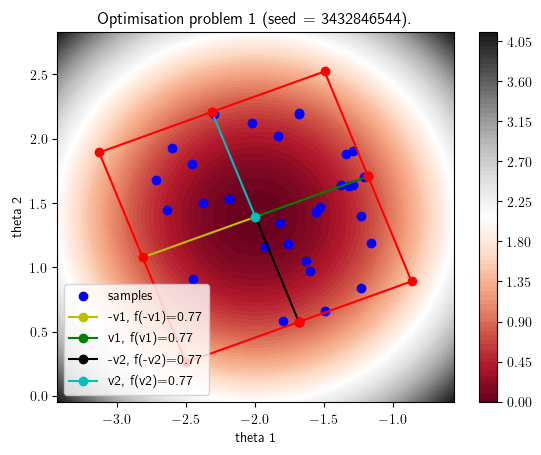
\includegraphics[width=0.48\textwidth]{./Thesis/images/chapter4/ex2D_region_1.png}
      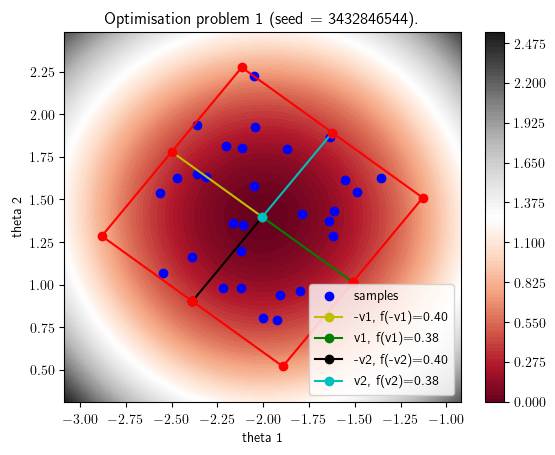
\includegraphics[width=0.48\textwidth]{./Thesis/images/chapter4/ex2D_region_1_bo.png}
    \end{center}
    \caption[2D example, the bounding box of the $1^{st}$ optimisation problem.]{The acceptance region and the bounding box of the
      $1^{st}$ optimisation problem; In the left plot, it is
      constructed with a gradient-based approach and in the right
      figure with Bayesian optimisation. We observe that both
      approaches construct a similar bounding box.}
  \label{fig:ex2_2}
\end{figure}


\begin{figure}[ht]
    \begin{center}
      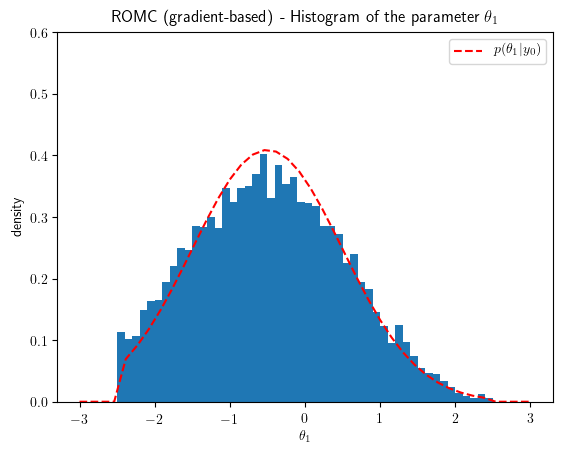
\includegraphics[width=0.48\textwidth]{./Thesis/images/chapter4/ex2D_hist_t1_romc.png}
      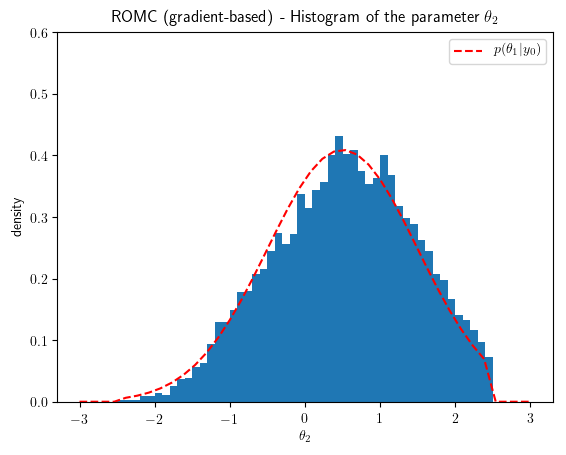
\includegraphics[width=0.48\textwidth]{./Thesis/images/chapter4/ex2D_hist_t2_romc.png}\\
      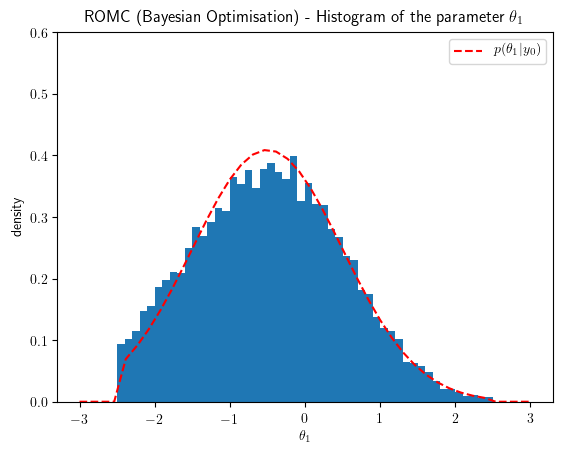
\includegraphics[width=0.48\textwidth]{./Thesis/images/chapter4/ex2D_hist_t1_romc_bo.png}
      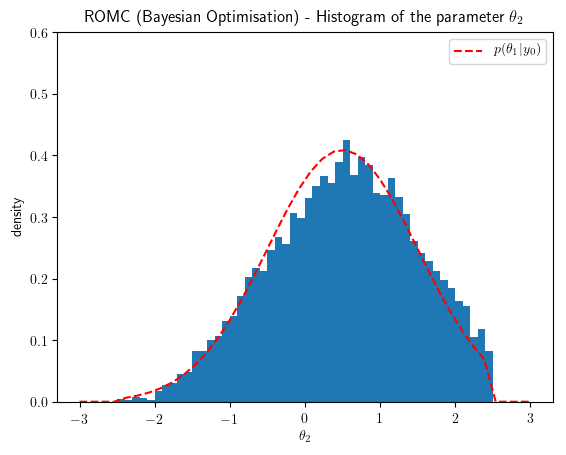
\includegraphics[width=0.48\textwidth]{./Thesis/images/chapter4/ex2D_hist_t2_romc_bo.png}\\
    \end{center}
    \caption[2D example, histogram of the weighted samples.]{Histogram of the weighted samples. The first row of plots
      refers to the gradient-based optimisation scheme, while the
      second row to the Bayesian optimisation. We represent the
      ground-truth marginal distribution $p(\theta_i|\data$ with the
      red dotted line. We observe that the samples follow the ground
      truth distribution quite accurately.}
  \label{fig:ex2_3}
\end{figure}

\begin{figure}[ht]
  \begin{center}
      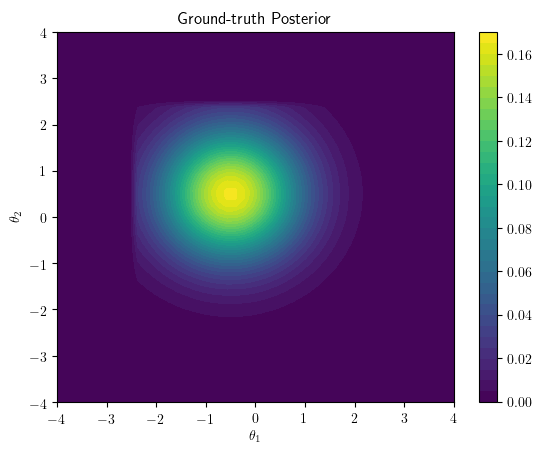
\includegraphics[width=0.5\textwidth]{./Thesis/images/chapter4/ex2D_gt_posterior.png}\\
      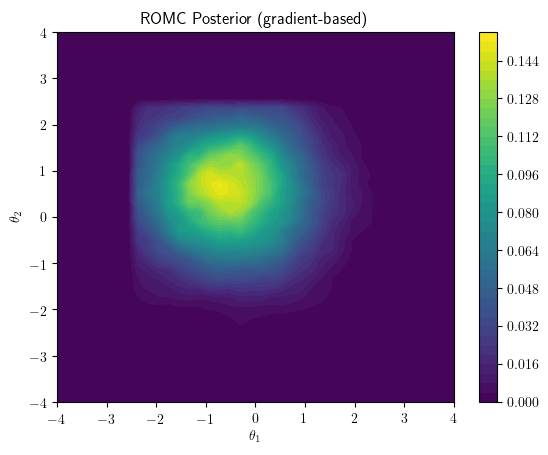
\includegraphics[width=0.48\textwidth]{./Thesis/images/chapter4/ex2D_romc_posterior.png}
      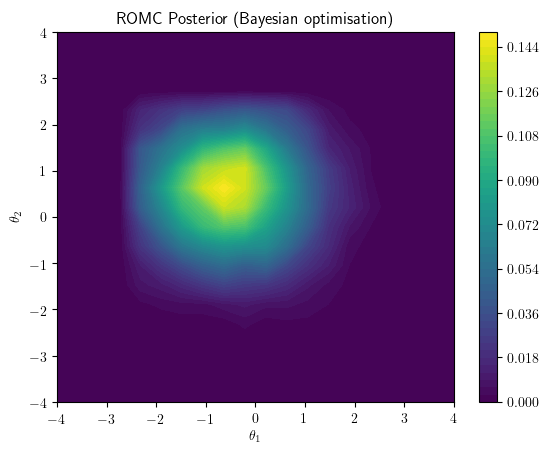
\includegraphics[width=0.48\textwidth]{./Thesis/images/chapter4/ex2D_romc_posterior_bo.png}
    \end{center}
    \caption[2D example, evaluation of the approximate posterior.]{(a) First row: Ground-truth posterior approximated
      computationally. (b) Second row (left): ROMC approximate
      posteriors using gradient-based approach. The divergence from
      the ground-truth using the Jensen-Shannon distance is
      $0.068$. (c) Second row (right): ROMC approximate posterior
      using Bayesian optimisation. The divergence from the
      ground-truth using the Jensen-Shannon distance is $0.069$}
  \label{fig:ex2_4}
\end{figure}

In this simple artificial 2D example, with the ground-truth
information available, we confirmed that our implementation produces
accurate approximations. In the following section, we will question it
in a more involved case.

